\documentclass[a4paper, 12pt, oneside]{article}

\usepackage[utf8]{inputenc}
\usepackage[T1]{fontenc}
\usepackage[french]{babel}
\usepackage{array}
\usepackage{shortvrb}
\usepackage{listings}
\usepackage[fleqn]{amsmath}
\usepackage{amsfonts}
\usepackage{fullpage}
\usepackage{enumerate}
\usepackage{graphicx}
\usepackage{subfigure}
\usepackage{alltt}
\usepackage{url}
\usepackage{indentfirst}
\usepackage{eurosym}
\usepackage{listings}
\usepackage{titlesec, blindtext, color}
\usepackage[table,xcdraw,dvipsnames]{xcolor}
\usepackage[unicode]{hyperref}
\usepackage{url}
\usepackage{float}
\usepackage{amsmath}
\usepackage{multicol}
\usepackage{amssymb}

\definecolor{mygray}{rgb}{0.5,0.5,0.5}

\lstset{
    language=C, % Utilisation du langage C
    commentstyle={\color{MidnightBlue}}, % Couleur des commentaires
    frame=single, % Entoure le code d'un joli cadre
    rulecolor=\color{black}, % Couleur de la ligne qui forme le cadre
    stringstyle=\color{RawSienna}, % Couleur des chaines de caractères
    numbers=left, % Ajoute une numérotation des lignes à gauche
    numbersep=5pt, % Distance entre les numérots de lignes et le code
    numberstyle=\tiny\color{mygray}, % Couleur des numéros de lignes
    basicstyle=\tt\footnotesize, 
    tabsize=3, % Largeur des tabulations par défaut
    keywordstyle=\tt\bf\footnotesize\color{Sepia}, % Style des mots-clés
    extendedchars=true, 
    captionpos=b, % sets the caption-position to bottom
    texcl=true, % Commentaires sur une ligne interprétés en Latex
    showstringspaces=false, % Ne montre pas les espace dans les chaines de caractères
    escapeinside={(>}{<)}, % Permet de mettre du latex entre des <( et )>.
    inputencoding=utf8,
    literate=
  {á}{{\'a}}1 {é}{{\'e}}1 {í}{{\'i}}1 {ó}{{\'o}}1 {ú}{{\'u}}1
  {Á}{{\'A}}1 {É}{{\'E}}1 {Í}{{\'I}}1 {Ó}{{\'O}}1 {Ú}{{\'U}}1
  {à}{{\`a}}1 {è}{{\`e}}1 {ì}{{\`i}}1 {ò}{{\`o}}1 {ù}{{\`u}}1
  {À}{{\`A}}1 {È}{{\`E}}1 {Ì}{{\`I}}1 {Ò}{{\`O}}1 {Ù}{{\`U}}1
  {ä}{{\"a}}1 {ë}{{\"e}}1 {ï}{{\"i}}1 {ö}{{\"o}}1 {ü}{{\"u}}1
  {Ä}{{\"A}}1 {Ë}{{\"E}}1 {Ï}{{\"I}}1 {Ö}{{\"O}}1 {Ü}{{\"U}}1
  {â}{{\^a}}1 {ê}{{\^e}}1 {î}{{\^i}}1 {ô}{{\^o}}1 {û}{{\^u}}1
  {Â}{{\^A}}1 {Ê}{{\^E}}1 {Î}{{\^I}}1 {Ô}{{\^O}}1 {Û}{{\^U}}1
  {œ}{{\oe}}1 {Œ}{{\OE}}1 {æ}{{\ae}}1 {Æ}{{\AE}}1 {ß}{{\ss}}1
  {ű}{{\H{u}}}1 {Ű}{{\H{U}}}1 {ő}{{\H{o}}}1 {Ő}{{\H{O}}}1
  {ç}{{\c c}}1 {Ç}{{\c C}}1 {ø}{{\o}}1 {å}{{\r a}}1 {Å}{{\r A}}1
  {€}{{\euro}}1 {£}{{\pounds}}1 {«}{{\guillemotleft}}1
  {»}{{\guillemotright}}1 {ñ}{{\~n}}1 {Ñ}{{\~N}}1 {¿}{{?`}}1
}

%%%% Page de garde %%%%

\title{\textbf{Introduction aux processus stochastiques}\\
	   Projet 1 : Analyse de la propagation d'un virus au sein d'un réseau}
\author{Maxime GOFFART \\180521 \and Olivier JORIS\\182113}
\date{Année académique 2019 - 2020}

\begin{document}

\maketitle
\newpage

\tableofcontents
\newpage

\section{Introduction}

\paragraph{}Les processus stochastiques permettent d'étudier des phénomènes aléatoires dans divers secteurs : l'économie, la climatologie, la météorologie, la biologie, \dotso

\paragraph{}Dans ce projet, il nous a été demandé d'étudier, en particulier, un phénomène d'actualité : la propagation d'un virus au sein d'un réseau, pouvant être modélisée à l'aide d'une chaîne de Markov. Ainsi, ce projet nous a permis d'appliquer les concepts vus au cours sur un exemple concret et d'actualité.

\section{Structure du programme} 
\paragraph{}Nous avons décidé de réaliser le projet en Python après comparaison des avantages et inconvénients des différents langages proposés. Notre code source se compose des fichiers suivants\footnote{Chaque méthode est décrite dans le module dans lequel elle est définie.} :

\begin{itemize}
	\item[$\bullet$] \texttt{exact\_model.py}: module principal pour l'étude du modèle exact à l'aide de la matrice de transition (section 1 de l'énoncé).
	\item[$\bullet$] \texttt{simulations\_study.py}: module principal pour l'étude sur base de simulations (section 2 de l'énoncé).
	\item[$\bullet$] \texttt{virus\_spread\_model.py}: module lié à la propagation du virus au sein de la population.
	\item[$\bullet$] \texttt{file\_management.py}: module qui permet de charger la matrice d'adjacence du graphe $W$ sous forme dense.
	\item[$\bullet$] \texttt{graphics\_generator.py}: module qui permet d'afficher le graphique des proportions des individus.
	\item[$\bullet$] \texttt{states\_manipulator.py}: module qui permet de manipuler les états d'une chaîne de Markov.
	\item[$\bullet$] \texttt{transition\_matrix.py}: module qui permet de manipuler la matrice de transition d'une chaîne de Markov.
\end{itemize}

\paragraph{}Nous avons utilisé différentes librairies externes\footnote{Aucune n'est spécifique aux chaînes de Markov comme mentionné sur eCampus.}. En voici la liste :

\begin{itemize}
	\item[$\bullet$] \texttt{Random} pour la génération de nombres pseudo-aléatoires.
	\item[$\bullet$] \texttt{Numpy} pour le produit matriciel et la puissance de matrices.
	\item[$\bullet$] \texttt{Matplotlib} pour l'affichage des graphiques.
\end{itemize}

\section{Étude du modèle exact}

\subsection{Question 1}
	
\paragraph{}Le modèle proposé dans l'énoncé est bien un processus de Markov en temps discret caractérisé par ses $3^N$ états \footnote{$N$ étant la taille de la population.}. Les états de cette chaîne sont caractérisés par la suite de longueur $N$ des catégories \footnote{S, R ou I.} auxquelles appartiennent les individus \footnote{Les individus étant indexés de 1 à N.} à l'instant t. Par exemple : pour $N = 3$, l'état "'S' 'I' 'I'" représente le fait que le premier individu est susceptible d'être infecté et que les deux derniers sont infectés.\\
\indent Les probabilités de transitions d'un état à un potentiel état de l'instant suivant de la chaîne dépendent à la fois de chacune des catégories des individus à l'instant initial et de leurs interactions avec des personnes infectées \footnote{Modélisées par le graphe $W$.}.\\
\indent Les états de cette chaîne, qui sont uniquement composés d'individus de la catégorie 'R' ou\footnote{Il s'agit d'un "ou" inclusif.} de la catégorie 'S', sont absorbants car la propagation du virus n'est plus possible s'il n'y a plus d'infectés. Il en va de même pour les états dans lesquels les infectés n'ont de contact avec personne\footnote{Cela correspond à une ligne remplie de 0 dans le graphe $W$.}. Cette chaîne n'est donc ni irréductible, ni régulière, ni périodique.

\subsection{Question 2}

\paragraph{}Soit $X$ une variable aléatoire, qui suit une distribution géométrique, représentant le temps de guérison d'un individu une fois qu'il a été infecté. On a: $$X \sim \mathcal{G}(\mu)$$ avec $\mu$ la probabilité de guérison.
\paragraph{}Le temps moyen nécessaire à un individu pour guérir une fois qu'il a été infecté est donné par l'espérance de $X$. On a: $$E(X) = \frac{1}{\mu}$$

\subsection{Question 3}

\paragraph{}Pour répondre à cette question, le programme peut-être lancé à l'aide de la commande suivante :

\begin{lstlisting}[language=bash]
$ python3 exact_model.py matrixSize fileName
\end{lstlisting}

\noindent où la première option spécifie la taille de la matrice $W$ utilisée et la deuxième représente le nom du fichier dans lequel cette matrice est encodée.

\subsubsection{Avec la matrice $W_{lin}$}

\paragraph{}Ainsi, en lançant le programme avec cette commande :

\begin{lstlisting}[language=bash]
$ python3 exact_model.py 6 6x6_lin.txt
\end{lstlisting}

\noindent On obtient ce graphique répondant à la première partie de la question avec les paramètres $\mu$ et $\beta$ fixés aux valeurs suggérées : 

\begin{figure}[H]
	\centering
	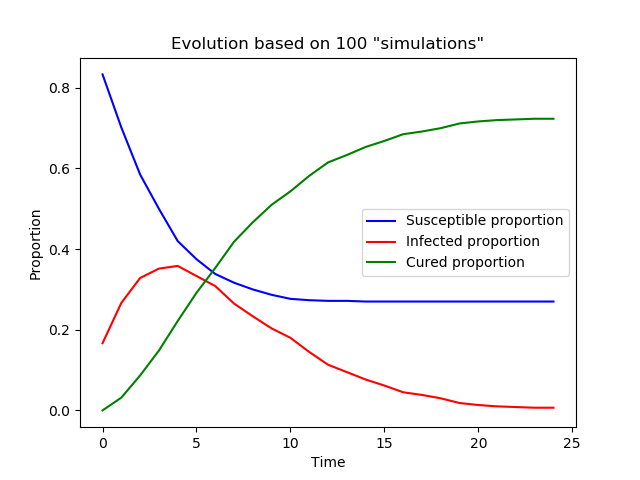
\includegraphics[scale=1]{lin_6x6.png} 
	\caption{Évolution des proportions d'individus dans chacune des catégories au cours du temps suivant un modèle représenté par une matrice $W_{lin}$.}
\end{figure}

\paragraph{}Sur la figure 1, on observe le fait que la proportion d'individus infectés est décroissante après une partie croissante jusque t $= 3$. En effet, les individus ayant peu de contacts les uns avec les autres, la probabilité qu'un individu soit infecté est faible.\\
De plus, les individus initialement infectés finissent par guérir. On observe, également, qu'une partie de la population reste "susceptible" d'obtenir le virus : elle ne l'a jamais contracté car les relations entre les individus sont limitées.

\subsubsection{Avec la matrice $W_{full}$}

\paragraph{}De la même façon en lançant le programme à l'aide de cette commande :
\begin{lstlisting}[language=bash]
$ python3 exact_model.py 6 6x6_full.txt
\end{lstlisting}

\noindent On obtient ce graphique répondant à la deuxième partie de la question avec les paramètres $\mu$ et $\beta$ fixés aux valeurs suggérées : 

\begin{figure}[H]
	\centering
	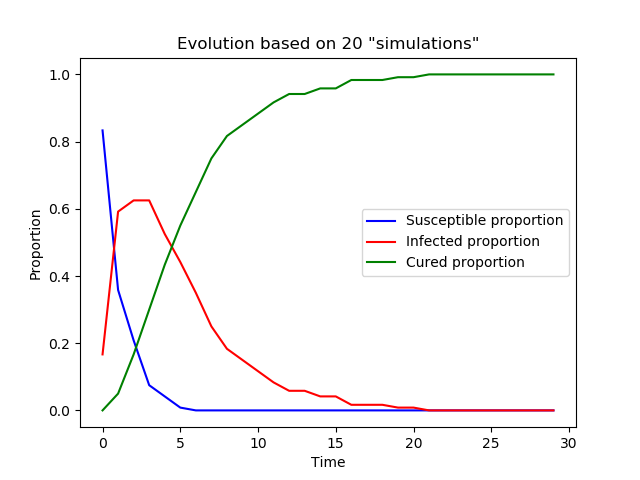
\includegraphics[scale=1]{full_6x6.png} 
	\caption{Évolution des proportions d'individus dans chacune des catégories au cours du temps suivant un modèle représenté par une matrice $W_{full}$.}
\end{figure}

\paragraph{}Sur la figure 2, on observe, à l'inverse de la situation précédente, que la population connaît un nombre important d'infectés et très rapidement car les gens sont tous en contact. On observe un pic en t $= 2$ avec une proportion de $\pm$ 77$\%$ d'infectés.\\
Au temps t = 4, on peut voir que la proportion d'individus susceptibles est proche de 0, c'est-à-dire que presque toute la population a été infectée à un instant inférieur ou égal à celui-ci. En effet, les individus ayant tous des contacts les uns avec les autres, le virus ne fait que se propager au sein de la population jusqu'à ce que celle-ci soit entièrement infectée.

\subsection{Question 4}

\paragraph{}Lors de l'exécution des deux précédentes commandes, le programme nous retourne également le temps nécessaire à la disparition du virus dans la population. Nous avons obtenu 34 dans le cas où les contacts entre les gens sont limités\footnote{Celui qui utilise la matrice $W_{lin}$.} et 33 dans l'autre cas\footnote{Celui qui utilise la matrice $W_{full}$.} avec une précision de 0.001. Nous n'avons pas directement accès aux états dans notre programme donc l'algorithme s'exécute jusqu'à atteindre 0 comme proportion d'individus infectés à une certaine précision près. Cette précision peut être modifiée dans le fichier \texttt{virus\_spread\_model.py} en modifiant la "constante" \texttt{PRECISION}.\\
Deux autres exécutions avec une précision égale à l'epsilon machine sur 32 bits ont donné 74 avec la matrice $W_{lin}$ et 73 avec l'autre matrice, $W_{full}$.
\paragraph{}On observe que le premier modèle\footnote{Celui dont la matrice d'adjacence est $W_{lin}$.} nécessite un temps légèrement supérieur au second avant la disparition du virus. Ceci s'explique par le fait que le virus se répand moins rapidement\footnote{Car les gens sont moins en contact les uns avec les autres.} donc, les gens qui sont infectés transmettent le virus à moins d'individus mais de nouvelles infections peuvent survenir plus tard et retardent ainsi la guérison de la population. Ce qui mène à la disparition du virus. Comme mentionné précédemment, une partie de la population n'est pas infectée par le virus.
\paragraph{}A l'inverse, dans le deuxième cas\footnote{Celui dont la matrice d'adjacence est $W_{full}$.}, le temps avant la disparition du virus est un peu plus court car l'entièreté de la population est rapidement atteinte donc, on peut très vite entrer dans une phase dans laquelle il faut guérir tout le monde.
\paragraph{}Cette petite différence de temps entre les 2 cas est contre intuitive. On s'attendrait à avoir un temps, dans le cas où les relations entre les individus sont représentées par $W_{lin}$, inférieur au temps dans le cas où les relations sont modélisées par $W_{full}$.\\
Comment expliquer cette erreur ? Une source d'erreurs potentielles est que les probabilités deviennent très faibles car on utilise des puissances d'une matrice remplie de nombres compris entre 0 et 1 et, dès lors, des erreurs de calculs peuvent survenir.

\section{Étude sur base de simulations}

\subsection{Question 1}

\paragraph{}L'hypothèse d'indépendance posée par les auteurs de l'article n'est, en général, pas vérifiée car la probabilité qu'un individu se trouve dans un état à un instant \textit{t} dépend en partie de son interaction avec les autres personnes de la population et de l'état de celles-ci à un instant précédent. Ainsi, si un individu, dans un état \textit{susceptible}, a des contacts avec des individus dans un état \textit{infectieux} alors, son état à un instant $t' > t$ sera impacté par ces derniers. L'indépendance n'est donc vérifiée que dans le cas où un individu n'a de contact avec personne.

\subsection{Question 2}

\paragraph{}Pour répondre à cette question, le programme peut-être lancé à l'aide de la commande suivante :
\begin{lstlisting}[language=bash]
$ python3 simulations_study.py populationSize fileName 
\end{lstlisting}
\noindent où la première option spécifie la taille de la matrice $W$ utilisée et la deuxième option correspond au nom du fichier dans lequel cette matrice est encodée.

\paragraph{}Ainsi, en lançant le programme avec cette commande :

\begin{lstlisting}[language=bash]
$ python3 simulations_study.py 6 6x6_lin.txt 
\end{lstlisting}

\noindent Le programme demande à l'utilisateur les paramètres que celui-ci souhaite utiliser pour les simulations. On choisit ainsi les valeurs suggérées dans l'énoncé. Ensuite, le script retourne le graphique de la figure 3 ainsi que le temps moyen de disparition des individus infectieux y correspondant\footnote{Étant ici d'environ 45 unités.}. On observe ainsi que l'étude sur base du modèle exact et celle sur base de simulations se ressemblent dans le cas où la matrice d'adjacence correspond à $W_{lin}$. Les différences observées peuvent être justifiées par le fait que les simulations n'utilisent pas la matrice de transition. Donc, la précision est plus faible par rapport au modèle exact.

\begin{figure}[H]
	\centering
	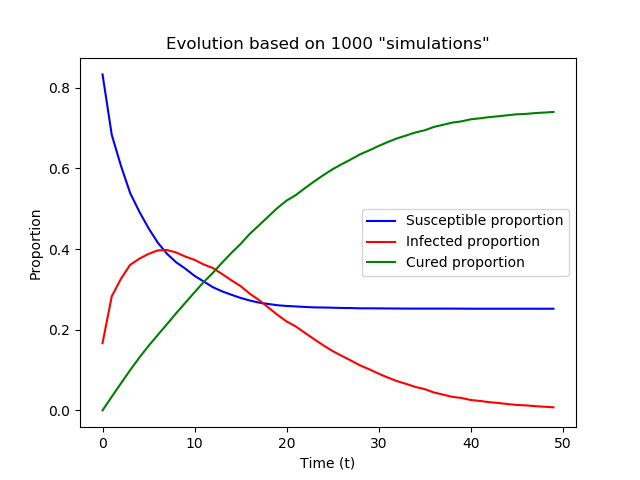
\includegraphics[scale=1]{lin_6x6_simulations.png} 
	\caption{Évolution des proportions d'individus dans chacune des catégories au cours du temps suivant un modèle représenté par une matrice $W_{lin}$ de taille $6 \times 6$.}
\end{figure}

\paragraph{}De la même façon en lançant le programme à l'aide de cette commande\footnote{Et en choisissant les paramètres suggérés dans l'énoncé.}:
\begin{lstlisting}[language=bash]
$ python3 simulations_study.py 6 6x6_full.txt 
\end{lstlisting}

\noindent On obtient le graphique de la figure 4 ainsi que le temps moyen de disparition des individus infectieux y correspondant\footnote{Valant ici environ 50 unités.}. On observe que l'étude sur base du modèle exact et celle sur base de simulations se ressemblent également dans ce cas de figure\footnote{Comme précédemment, les différences peuvent s'expliquer par le fait que les simulations n'utilisent pas la matrice de transition. Donc, la précision est plus faible.}. On peut donc penser que cette simulation approxime de manière satisfaisante la réalité et permettrait ainsi de modéliser cette même simulation avec une population plus nombreuse\footnote{En prenant un nombre de simulations suffisamment grand pour que les calculs soient stables.}.

\begin{figure}[H]
	\centering
	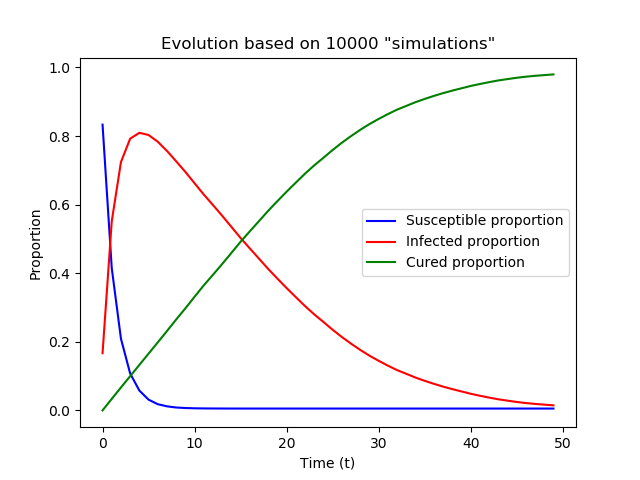
\includegraphics[scale=1]{full_6x6_simulations.png} 
	\caption{Évolution des proportions d'individus dans chacune des catégories au cours du temps suivant un modèle représenté par une matrice $W_{full}$ de taille $6 \times 6$.}
\end{figure}

\subsection{Question 3}

\paragraph{}En lançant le programme à l'aide de la commande suivante\footnote{En choisissant un nombre suffisant de simulations pour avoir des résultats stables.} :

\begin{lstlisting}[language=bash]
$ python3 simulations_study.py 2000 Wbig_dense.txt 
\end{lstlisting}

\noindent Le programme retourne le graphique de la figure 5 ainsi que le temps moyen de disparition des individus infectieux y correspondant\footnote{Étant ici d'environ 10 000 unités.} avec les probabilités $\beta$ et $\mu$ fixées au valeurs suggérées.

\begin{figure}[H]
	\centering
	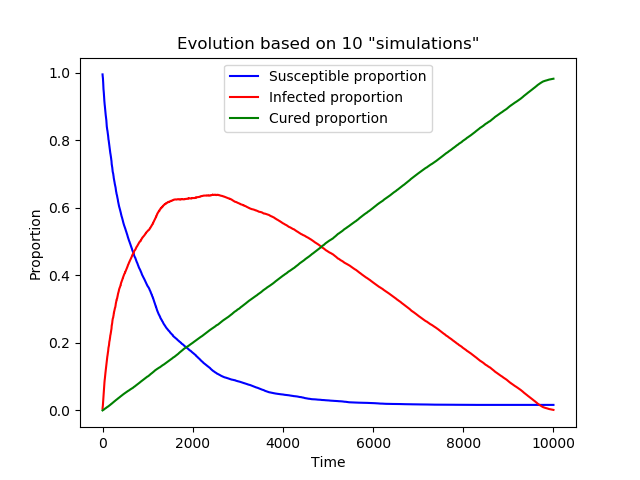
\includegraphics[scale=1]{Wbig_dense_simulations.png} 
	\caption{Évolution des proportions d'individus dans chacune des catégories au cours du temps suivant un modèle représenté par une matrice d'adjacence $W_{big}$ de taille $2000 \times 2000$ générée aléatoirement selon un modèle "scale-free" quand aucune mesure de sécurité n'est prise.}
\end{figure}

\subsection{Question 4}

\paragraph{}Si le graphique de la figure 5 représente l'évolution de l'épidémie dans le cas où aucune mesure n'est prise, étudions l'impact des mesures suivantes :

\paragraph{}(a) Réduire la probabilité de transmission de la maladie via différents moyens revient à diminuer la probabilité de contamination $\beta$. Ainsi, en réduisant la probabilité $\beta$ à 0.2, on obtient le graphique de la figure 6 qui permet de visualiser que cette mesure permet d'avoir une proportion de la population qui n'est pas infectée par le virus. De plus, le temps de disparition de ce dernier diminue\footnote{Valant ici environ 8300}.

\begin{figure}[H]
	\centering
	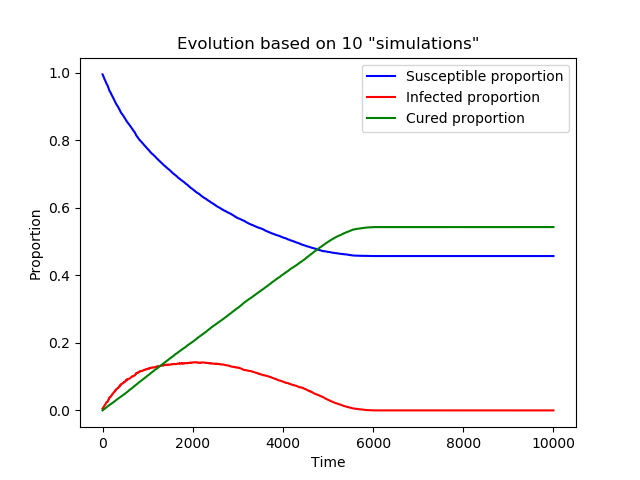
\includegraphics[scale=1]{Wbig_dense_reduction_transmission.png} 
	\caption{Évolution des proportions d'individus dans chacune des catégories au cours du temps suivant un modèle représenté par une matrice d'adjacence $W_{big}$ de taille $2000 \times 2000$ générée aléatoirement selon un modèle "scale-free" avec une probabilité de transmission de la maladie réduite : $\beta = 0.2$.}
\end{figure}


\paragraph{}(b) Réduire les interactions entre les individus revient à diminuer le nombre de 1 dans la matrice $W_{big}$. En imposant un maximum d'interactions égal à 6 par personne par rapport à la matrice initiale, on obtient le graphique de la figure 7 montrant que cette mesure permet également d'accélérer la stabilisation de la situation\footnote{Le temps de stabilisation valant ici environ 8000.} et de réduire la proportion d'infectés.

\begin{figure}[H]
	\centering
	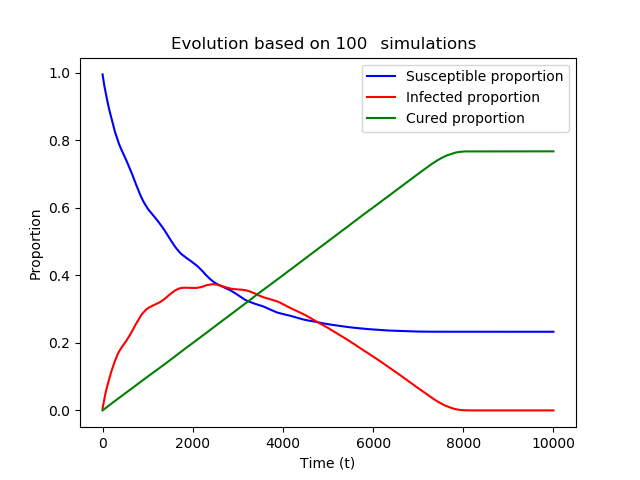
\includegraphics[scale=1]{Wbig_dense_containment.png} 
	\caption{Évolution des proportions d'individus dans chacune des catégories au cours du temps suivant un modèle représenté par une matrice d'adjacence $W_{big}$ de taille $2000 \times 2000$ générée aléatoirement selon un modèle "scale-free" avec des mesures de confinement prises telles qu'une personne a au maximum 6 interactions physiques avec d'autres personnes du modèle initial.}
\end{figure}

\paragraph{}(c) Vacciner un certain pourcentage de la population correspond à ajouter cette proportion d'individus dans l'état 'R' à l'instant $t = 0$. Le graphique de la figure 8 représente la situation où 30\% de la population est vaccinée. Celui-ci permet également d'avoir une proportion d'individus qui n'est jamais infectée et de réduire le temps de disparition du virus\footnote{Le temps de stabilisation de la situation passant ici à environ 6000.}.

\begin{figure}[H]
	\centering
	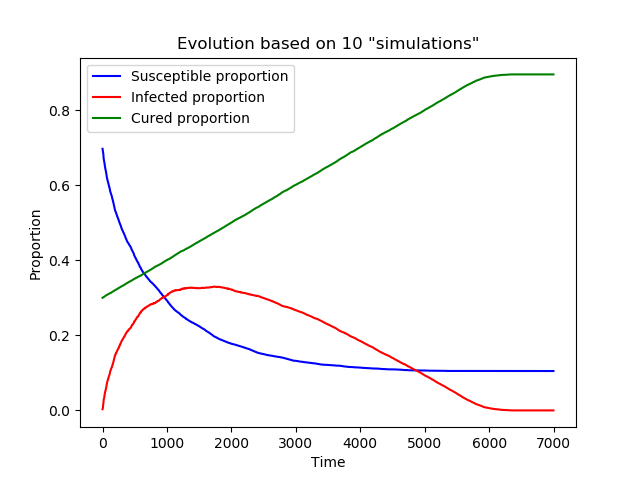
\includegraphics[scale=1]{Wbig_dense_initial_immunised.png} 
	\caption{Évolution des proportions d'individus dans chacune des catégories au cours du temps suivant un modèle représenté par une matrice d'adjacence $W_{big}$ de taille $2000 \times 2000$ générée aléatoirement selon un modèle "scale-free" avec une proportion de 30\% d'individus vaccinés.}
\end{figure}

\paragraph{}(d) Traiter les patients avec un médicament qui permettrait d'accélérer la guérison revient à augmenter la probabilité de guérison $\mu$. En augmentant la probabilité de guérison à 0.5, on voit sur la figure 9 que la principale amélioration est la vitesse de disparition du virus\footnote{Le temps de disparition du virus étant ici égal à environ 3600.}. On remarque également qu'une proportion d'individus ne se fait pas infecter.

\begin{figure}[H]
	\centering
	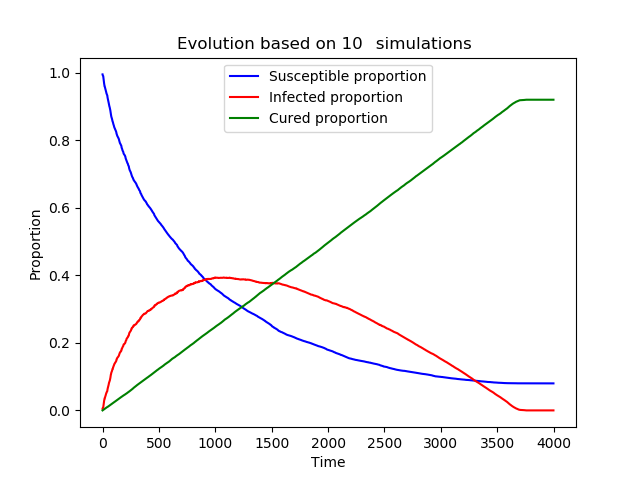
\includegraphics[scale=1]{Wbig_dense_speeded_heal.png} 
	\caption{Évolution des proportions d'individus dans chacune des catégories au cours du temps suivant un modèle représenté par une matrice d'adjacence $W_{big}$ de taille $2000 \times 2000$ générée aléatoirement selon un modèle "scale-free" avec une accélération de guérison : $\mu = 0.5$.}
\end{figure}

\subsubsection{Comparaison des différentes mesures}

\paragraph{}Si on fixe un nombre de lits disponibles pour une hospitalisation à 13, soit 6,5 lits pour 1000 habitants\footnote{Source : \url{https://www.indexmundi.com/fr/belgique/lits_d_hopitaux_par_habitant.html}.} et que l'on suppose que 5\% des personnes infectées ont besoin d'être hospitalisées, cela revient ainsi à veiller à avoir une proportion d'infectés ne dépassant pas $\frac{13}{2000 \times 0,05} = 0.13$. Voici les valeurs minimales des différentes mesures à prendre :

\paragraph{}(a) Pour cette mesure, il faut arriver à réduire la probabilité de transmission à 0.09. Dans ce cas on obtient le graphique de la figure 10.

\begin{figure}[H]
	\centering
	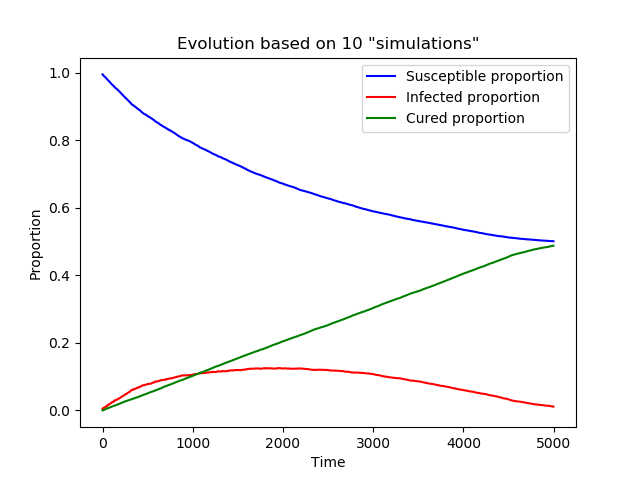
\includegraphics[scale=1]{Wbig_dense_reduction_transmission_comparaison.png} 
	\caption{Évolution des proportions d'individus dans chacune des catégories au cours du temps suivant un modèle représenté par une matrice d'adjacence $W_{big}$ de taille $2000 \times 2000$ générée aléatoirement selon un modèle "scale-free" avec une probabilité de transmission de la maladie réduite : $\beta = 0.09$ .}
\end{figure}

\paragraph{}(b) Il faut ici réduire les contacts entre individus de façon à avoir maximum 3 contacts par individus\footnote{En partant de la matrice $W$ initiale, c'est-à-dire que si une personne avait moins de 3 interactions, de nouvelles ne sont pas créées.}. Le résultat correspondant est représenté sur le graphique de la figure 11.

\begin{figure}[H]
	\centering
	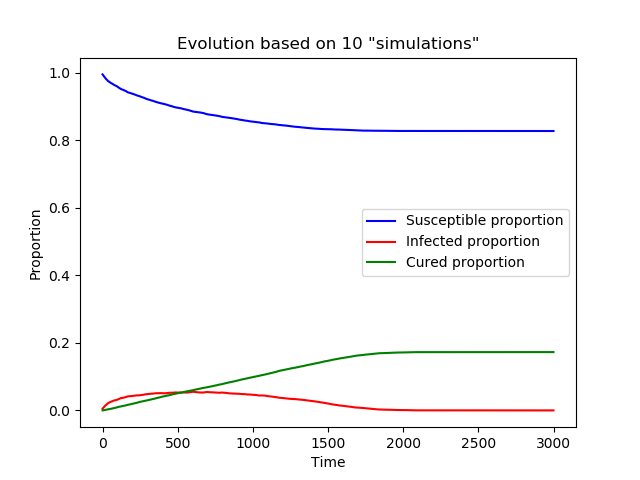
\includegraphics[scale=1]{Wbig_dense_containment_comparaison.png} 
	\caption{Évolution des proportions d'individus dans chacune des catégories au cours du temps suivant un modèle représenté par une matrice d'adjacence $W_{big}$ de taille $2000 \times 2000$ générée aléatoirement selon un modèle "scale-free" avec des mesures de confinement prises telles qu'une personne a au maximum 3 interactions physiques avec d'autres personnes du modèle initial.}
\end{figure}

\paragraph{}(c) Il faut qu'initialement environ 55\% de la population soit vaccinée pour respecter la limite de lits d'hôpitaux disponibles, le graphique de la figure 12 représente cette situation.

\begin{figure}[H]
	\centering
	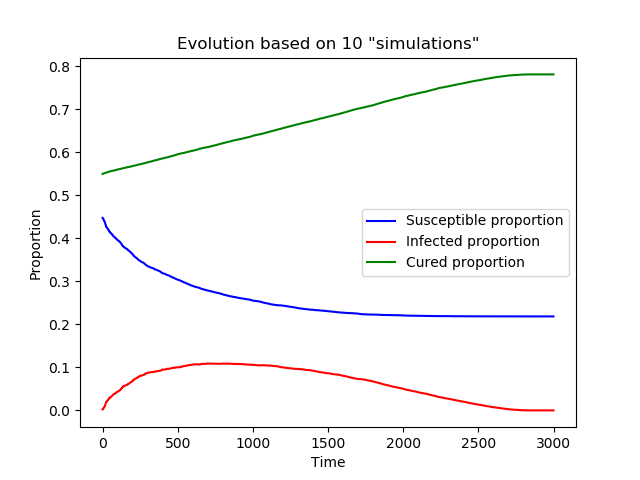
\includegraphics[scale=1]{Wbig_dense_initial_immunised_comparaison.png} 
	\caption{Évolution des proportions d'individus dans chacune des catégories au cours du temps suivant un modèle représenté par une matrice d'adjacence $W_{big}$ de taille $2000 \times 2000$ générée aléatoirement selon un modèle "scale-free" avec une proportion initiale d'individus vaccinés de 55\%.}
\end{figure}

\paragraph{}(d) Enfin, en faisant passer la probabilité $\mu$ de guérison à 1, le nombre de lits d'hôpitaux disponibles est quand même dépassé. Ceci peut être observé sur la figure 13.

\begin{figure}[H]
	\centering
	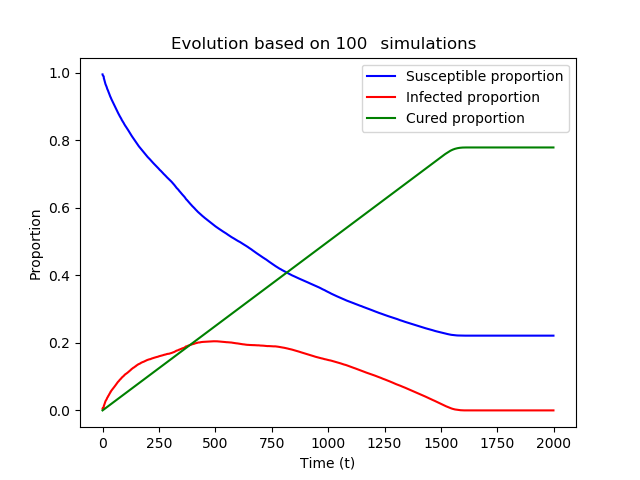
\includegraphics[scale=1]{Wbig_dense_speeded_heal_comparaison.png} 
	\caption{Évolution des proportions d'individus dans chacune des catégories au cours du temps suivant un modèle représenté par une matrice d'adjacence $W_{big}$ de taille $2000 \times 2000$ générée aléatoirement selon un modèle "scale-free" avec une accélération de la guérison du virus : $\mu = 1$.}
\end{figure}

\paragraph{} On peut enfin comparer le temps de disparition du virus selon les différentes mesures prises. On obtient ainsi ce classement de durée décroissante : $(a) > (c) > (b) > (d)$. On conclut donc que la mesure (d) a pour principal effet de diminuer la durée de l'épidémie mais pas spécialement la proportion d'individus infectés. Cette mesure pourrait donc être prise quand la maladie n'est pas importante et qu'il n'y a donc besoin d'hospitalisation que pour une proportion négligeable de la population. Les autres mesures\footnote{Pouvant être combinées les unes avec les autres.} ont à la fois l'avantage de diminuer la proportion d'individus infectés et le temps de disparition du virus.

\end{document}
